\subsubsection{Track}

The ATLAS detector is composed of two independent tracking systems: the Inner Detector (ID) close to the interaction point, and the Muon Spectrometer (MS).
The reconstructed charged-particle trajectories in the ID and MS are referred to as ID tracks and MS tracks respectively.
The ID reconstruction needs to handle high track density that imposes a large number of combinatorial track candidates, 
the MS reconstruction is however largely limited by the huge amount of inert material, the large background and the highly inhomogeneous magnetic field\cite{Cornelissen:1020106}.
More details of two types of track reconstructions are given below.

\textbf{Inner detector track}

Figure~\ref{fig:track_ID} shows the ID system used for detect charge-particle tracks.
The ID track revonstructions contains two sequences: \textit{inside-out} track reconstruction and \textit{outside-in} one.
\begin{figure}[!htb]
  \centering
  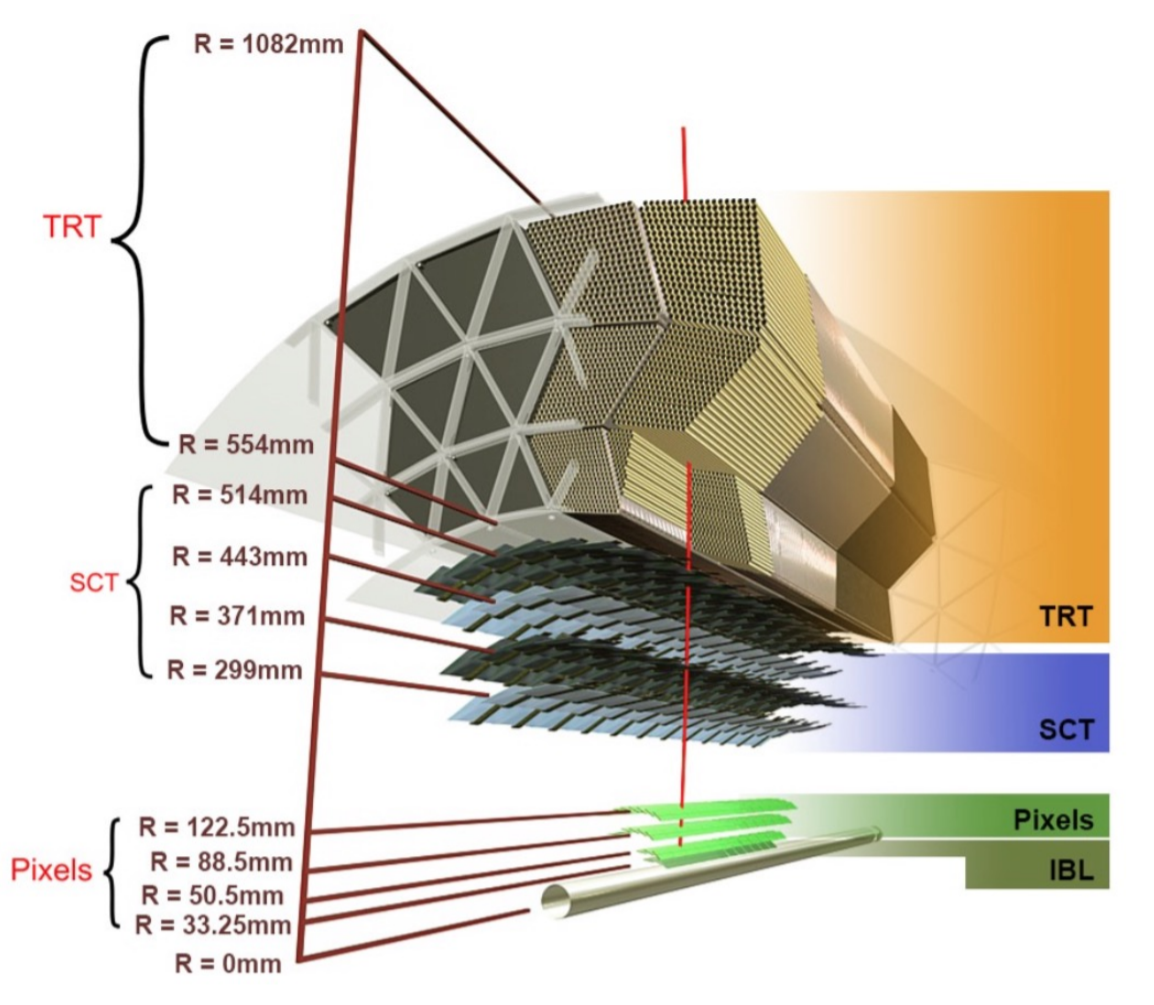
\includegraphics[width=0.7\textwidth]{figures/Simulation/track_ID.png}
  \caption{Schematic view of the ATLAS inner detector showing all the corresponding components.}
  \label{fig:track_ID}
\end{figure}

For inside-out tracking, it exploits the high granularity of the pixel and SCT detectors to discover prompt tracks originating from the interaction point.
In first step, the track seeds are formed by combining the information of space-points in the three pixel layers and the first SCT layer.
Then, these seeds are extended throughout the SCT to build track candidates.
After that, these candidates are fitted, some quality cuts are applied to remove the outlier clusters, reject the fake tracks and resolve ambiguities in the cluster-to-track association.
The selected tracks are then further extended to TRT, and refitted with the full information from pixel, SCT and TRT detectors.

Another complementary approach, ouside-in, searches for unused track segments start from TRT instead.
These segments are then extended into the SCT and pixel detectors to improve the tracking efficiency for secondary tracks from conversions or decays of long-lived particles.

\textbf{Muon spectrometer track}

The MS track reconstruction\cite{Aad:2016jkr} starts from searching hit patterns inside each muon chamber to form segments.
In each MDT chamber and nearby trigger chamber, a Hough transform\cite{ILLINGWORTH198887} is used to search the hits lies on a certain trajectory in the bending plane of the detector.
The MDT segments are reconstructed by performing a linear fit to the hits found in each layer.
The RPC or TGC hits can be built by measuring the coordinate orthogonal to the bending plane.
And the segments of CSC can be built using a separate combinatorial search in the $\eta$ and$\phi$ detector planes.
